%!TEX root = main.tex
\chapter{Instalación de herramientas}

Este apéndice esta dedicado al proceso de instalación de las herramientas que permiten la generación del compilador \Set en las plataformas Ubuntu Linux, OS X y Windows. Las herramientas necesarias son cuatro:
\begin{itemize}
	\item el generador de analizadores léxicos, \emph{Flex}; 
	
	\item el generador de analizadores sintácticos, \emph{Bison};

	\item la herramienta para el control de la recompilación, \emph{Make} y 

	\item el compilador del lenguaje C++, \emph{GNU C++} (g++)\footnote
	{
		g++ es el alias tradicional de «GNU C++» un conjunto gratuito de compiladores de C++. Forma parte del GCC, «GNU Compiler Collection» (del inglés, colección de compiladores GNU).
	}.
\end{itemize}

\section{Linux}

	En los sistemas operativos basados en Linux la instalación se suele realizar desde el shell (terminal)\footnote
	{
		Al shell también se le conoce como intérprete de órdenes o línea de comandos.
	}
	de la siguiente manera:
	\begin{enumerate}
		\item Asegúrese de que está conectado a Internet.

		\item Abra una ventana de terminal pulsando la combinación de teclas \pat{Ctrl+Alt+T} o pase al modo consola virtual pulsando la combinación \pat{Ctrl+Alt+F1}\footnote
		{
			En el modo de consola virtual el terminal se abre a pantalla completa, es decir, desaparece la GUI (interfaz gráfica de ususario) y es necesario escribir el nombre de usuario y la contraseña antes de insertar los comandos para la instalación de las herramientas.
		}.
		Otra forma de abrir un terminal en Ubuntu es haciendo clic con el botón izquierdo del ratón sobre el botón \pat{Inicio} (figura~\ref{subfig:ubuntu_boton_inicio}) y donde aparece \pat{Buscar} (figura~\ref{subfig:ubuntu_buscador}) escriba \pat{terminal} (figura~\ref{subfig:ubuntu_terminal}), por último haga clic con el botón izquierdo sobre el icono del terminal.
		\begin{figure}[!ht]
			\subfloat[Botón de inicio de Ubuntu\label{subfig:ubuntu_boton_inicio}]%
			{%
     			 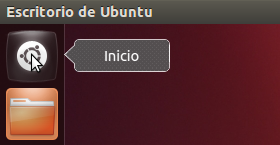
\includegraphics[width=0.45\textwidth]{ubuntu_boton_inicio}
    		}
    		\hfill
    		\subfloat[Buscador de Ubuntu\label{subfig:ubuntu_buscador}]%
    		{%
      		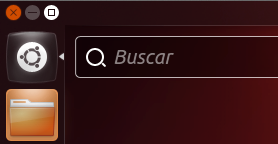
\includegraphics[width=0.45\textwidth]{ubuntu_buscador}
      	}
      	\hfill\centering
    		\subfloat[Icono del terminal de Ubuntu\label{subfig:ubuntu_terminal}]%
    		{%
      		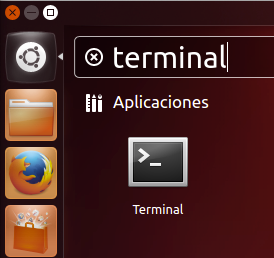
\includegraphics[width=0.4\textwidth]{ubuntu_terminal}
      	}
      	\caption{Apertura de un terminal en Ubuntu}
    		\label{fig:apertura_terminal_ubuntu}
    	\end{figure}

		\item Para instalar Flex escriba el siguiente comando en la terminal y pulse la tecla enter:

		\cod{sudo apt-get install flex}

		\fbox{\parbox{\linewidth}{\small Siempre que, durante la instalación de una herramienta, se le pregunte \pat{¿Desea continuar [S/n]?} escriba una \pat{S} mayúscula y pulse enter (figura~\ref{fig:ubuntu_instalacion_flex}).}}
		\begin{figure}[!ht]
			\centering
			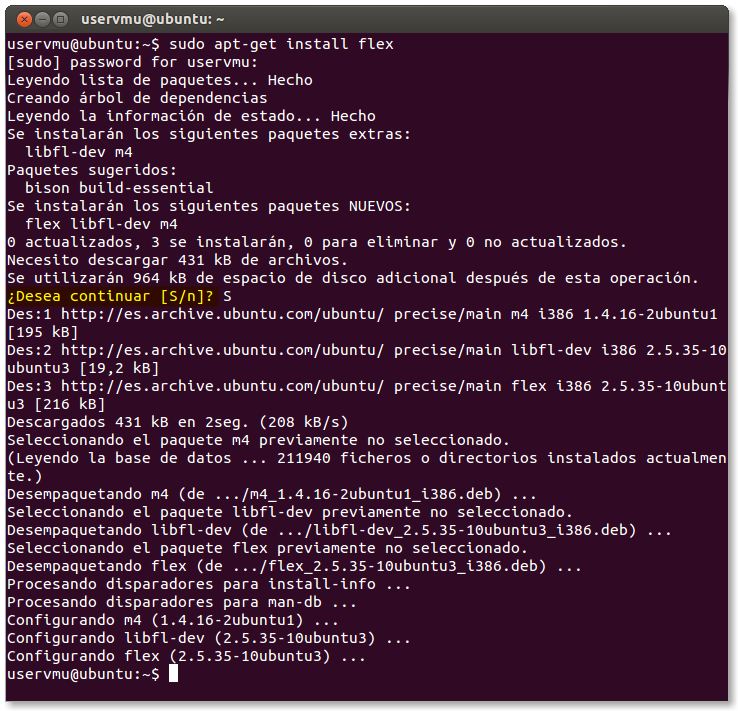
\includegraphics[width=0.85\textwidth]{ubuntu_instalacion_flex}
			\caption{Instalación de Flex en Ubuntu mediante el shell}
			\label{fig:ubuntu_instalacion_flex}
		\end{figure}

		\item Para instalar Bison escriba el siguiente comando y pulse enter:

		\cod{sudo apt-get install bison}

		\item Para instalar g++ escriba el siguiente comando y pulse enter:

		\cod{sudo apt-get install g++}

		\item La herramienta Make viene instalada por defecto en la mayoría de los sistemas basados en Linux. Si por casualidad su sistema no le proveyera dicha herramienta, puede utilizar el siguiente comando para instalarla:

		\cod{sudo apt-get install make}
	\end{enumerate}

	Otro modo de instalación es usando el centro de software de ubuntu.

\section{OS X}

	En los sistemas OS X puede obtener todas las herramientas necesarias instalando el IDE (entorno de desarrollo integrado) Xcode

	El IDE Xcode ocupa un espacio considerable (más de 5 GiB), puede obtener una instalación más liviana de las herramientas necesarias utilizando MacPorts \url{http://www.macports.org/ports.php?by=name&substr=gcc}

\section{Windows}

